% switch the class for review format
\documentclass[lettersize,journal,onecolumn]{IEEEtran}
%\documentclass[lettersize,journal]{IEEEtran}

\usepackage{amsmath,amsfonts}
\usepackage{algorithmic}
\usepackage{array}
\usepackage[caption=false,font=normalsize,labelfont=sf,textfont=sf]{subfig}
\usepackage{textcomp}
\usepackage{stfloats}
\usepackage{epstopdf}
\usepackage{url}
\usepackage{verbatim}
\usepackage{graphicx}
\usepackage{paracol}
\hyphenation{op-tical net-works semi-conduc-tor IEEE-Xplore}
\def\BibTeX{{\rm B\kern-.05em{\sc i\kern-.025em b}\kern-.08em
    T\kern-.1667em\lower.7ex\hbox{E}\kern-.125emX}}
\usepackage{balance}
\begin{document}
\title{Robotic Reconstruction of Islamic Calligraphy Using Twisting Bezier Splines}
\author{Muhammad Umar Hassan, Muhammad Sabieh Anwar and Ali Raza
%\thanks{Manuscript created October, 2020; This work was developed by the IEEE Publication Technology Department. This work is distributed under the \LaTeX \ Project Public License (LPPL) ( http://www.latex-project.org/ ) version 1.3. A copy of the LPPL, version 1.3, is included in the base \LaTeX \ documentation of all distributions of \LaTeX \ released 2003/12/01 or later. The opinions expressed here are entirely that of the author. No warranty is expressed or implied. User assumes all risk.}
}

\markboth{IEEE Robotics and Automation Letters}%
{How to Use the IEEEtran \LaTeX \ Templates}

\maketitle

\author{Muhammad Umar Hassan, Muhammad Sabieh Anwar and Ali Raza}
% uncomment to enable review format
%\begin{paracol}{2}
%    \switchcolumn[0]
    \begin{abstract}
\label{Chapter:Abstract}
{
    Automated reconstruction of Islamic architectural calligraphy can save thousands of nobel and historic scripts all over the world from going extinct. One of the fundamental problems in such reconstruction tasks is the absence of a tool that can bridge the gap between artists and the machines (such as a robotic arms) by taking input as conventional calligraphy format and transform into a robot-program. Not just the reconstruction, even in this digital age, no such method exists that lets the artists generate new broad-edge scripts that can be reproduced mechanically. In this context, the research presented herein introduces a novel innovation in the conventional Bezier spline curves to use them to effectively answer the artistic requirements of copying or creating broad-edge calligraphy scripts and can directly produce data needed by the industrial robots. To demonstrate the effectiveness of our approach, two famous scripts are reproduced using the new splines and a comparison is made with the originals. Additionally, to establish how these splines can be used with machines, a robotic simulator is also discussed and the output analyzed both qualitatively and quantitatively. In addition to mechanized reconstruction Islamic calligraphy, the presented approach can also be used for generating calligraphy for virtual 3D models, e.g. in Metaverse, and 3D documentation of non-reachable and ruined buildings.
}
\end{abstract}

    \begin{IEEEkeywords}
    Art and Entertainment Robotics, Motion Control, Human-Centered Automation, Software Tools for Robot Programming
    \end{IEEEkeywords}
    \input{03 - Introduction.tex}
    \section{Rotating/Twisting Bezier Splines}
\label{Chapter:SplineModelling}

    \subsection{The need of a Twisting Bezier splines}

    Conventional Bezier curves are commonly used to define outline fonts [cite] and digital calligraphy [cite] due to their ability to accurately trace [cite] the outline of scripts written with and without a broad edge tool [cite]. These curves can be easily manipulated [cite] and rendered [cite] on a computer screen as well as they can be printed on paper. However, in light of the underlaying problem, it is desired that a script is written using a conventional broad-edge tool by a robotic manipulator [cite] in a similar fashion a human artist would have used in order to preserve the essence of artistic norms [cite]. Separate techniques [cite] are needed to convert output of the outline or pitch curve functions to a format that a robot can directly use to for the required tool movement. Even though many of these techniques [cite] can promise accurate tracing, none of them can promise an exact tool movement that a human would like to use.

    In the most literal terms, beizer spline curves are sets of decimal values that define the graphical shape of certain mathematical functions [cite]. The input of these functions contains two dimensional points located in the frame of reference of the screen on which they are created and work as handles to control the shape of the curve. A user can physically relocate these curvature handles on the computer screen and the shape of the resulting spline will follow. The output of these mathematical functions is absolutely repeatable and can be linearly scaled to any units. Usually, a curve is made of up a lot of such lines each with its own set of input coefficients. Although these individual functions are continuous, there output can easily be discretized as closed paths made up of closely located two dimensional points with controllable resolution [cite]. This is exactly the kind of information required by most of computer graphics and printing drivers to render an output.

    Now, as effective as the bezier curves are for screen and paper printing, they still cannot tell how a physical tool should move on a piece of paper to create the desired output. The splines are just organic shaped paths with no thickness. To convert them into ink-mark, one way to interpret them is to consider them as a pitch line for a thick round tool tip. This technique is used by plotters [cite] and some hand writing replicators [cite] to produce a written script. However, only a few fonts [cite] can be replicated by this technique. The other technique is to fill the glyph by moving the tool continuously on a path computed by algorithms such as those used by CAD tools [cite] to fill in the area contained by the outline of the glyph using a round tip tool. The later can produce outputs that looks similar to broad-edge calligraphy but will still not be the same due to the visible tool paths that are not expected when using an actual broad edge tool.

    Conventionally, image processing is being used to extract data that can be used to create machine data. We, however, propose a difference; no matter how strong and robust image processing gets, we maintain that there is no alternative to the minor details only a real artist can observe and recreate. So a solution is needed that fulfils the technical needs as well as the artistic demands. One can virtually draw any kind of shape that can be represented on a two dimensional surface using the conventional bezier splines but it is not very intuitive to accurately reproduce the output of a broad-edge tool.

    Twisting bezier splines bridge this gaps by introducing a small but important innovation in the conventional bezier spline curves. Instead of working as outline curves, they directly record the pitch line of a twisting broad-edge tool stroke along-with the twist information of the tool. Their usage is just as intuitive as the conventional bezier splines and will be demonstrated in the next chapters, and the information they poses can not only be used to render the script back on the screen or a photo printer, but also be directly considered as machine data for robotic manipulators.

    On the other hand, for a particular glyph created with a broad edge, the twisting bezier spline curves not only trace the pitch lines of all the strokes but also the twist of the tool independent of the curvature. This is done by introducing another input to the curve function we call the ``Rotation/Twist'' handle. Just like the curvature handles represent the function inputs responsible to define the curvature, the rotation handles represent the inputs that controls the twist of the simulated broad-edge tool. Just like the conventional bezier splines, the functions of the twisting bezier splines can also be discretized and converted into a list of two dimensional list of points; a closed path to emulate the ink-mark of the broad edge tool, exactly the kind of data needed by the computer display drivers. This is how an artist can intuitively use the twisting curves not just to trace but also to create calligraphy that is not bound by any culture or language.

    The interesting part is that, logically, the twisting beizer splines are more near to the machine than they are to computer graphics data. To compute the list of the points needed to create a filled path that represents the ink-mark, a broad edge tool is emulated to be moving on the rotating spline with the twist also controlled by the spline. In actuality, the emulated tool is replaced by an actual tool that can be mounted on a robotic manipulator. The spline directly controls the position and twist of the tip of a tool which can directly be translated into machine movement codes. The rest of the process for painting involves inverse kinematics and is already handled by the robot controller.

    As discussed in section \ref{Chapter:Problem Statement}, the first part of the main problem is extracting digital machine data from the existing calligraphy specimens. Conventionally, image processing is being used to extract data that can be used to create machine data. We, however, propose a difference; no matter how strong and robust image processing gets, we maintain that there is no alternative to the minor details only a real artist can observe and recreate. So a solution is needed that fulfils the technical needs as well as the artistic demands.

    \subsection{Mathematical Model of a Rotating Bezier Spline}
    \subsubsection{The Conventional Bezier Spline}
         To describe how twisting splines work, we, once again, first describe it for a conventional bezier spline. Figure \ref{Fig:BezierSplines} shows an illustration of a spline path made up of several sub curves. Each curve section is only partly independent of the other. Figure \ref{Fig:BezierSplines} (a) shows the final shape of the curve without any construction elements. In Figure \ref{Fig:BezierSplines} (b), we explode different sections of the curve into smaller elements and show how they fit together to form the complete spline. There are five sections in this curve labeled $1$ through $5$. Figure \ref{Fig:BezierSplines} (c) shows an assembled form of these five sections. It also shows, what are called, anchors and construction handles. The anchor is the point that sits at the terminals of two adjacent curve sections. For instance, anchor point $A$  is connecting the sections $1$ and $2$. Like all the other anchors, this anchor also has two handles, $H_1$ and $H_2$, connected through a straight line passing through the anchor. The length of each handles, $\overline{AH_1}$  and $\overline{AH_2}$ on both sides of the anchor define the shape of the curve section on their respective side where as the orientation of line connecting both handles contributes to the shape on both the curve sections. This is how both sections become partly independent. For instance, handle $\overline{AH_1}$ contributes to the shape of curve segment $1$ and $\overline{AH_1}$ to section $2$.



        \begin{figure}[!t]
            \centering
            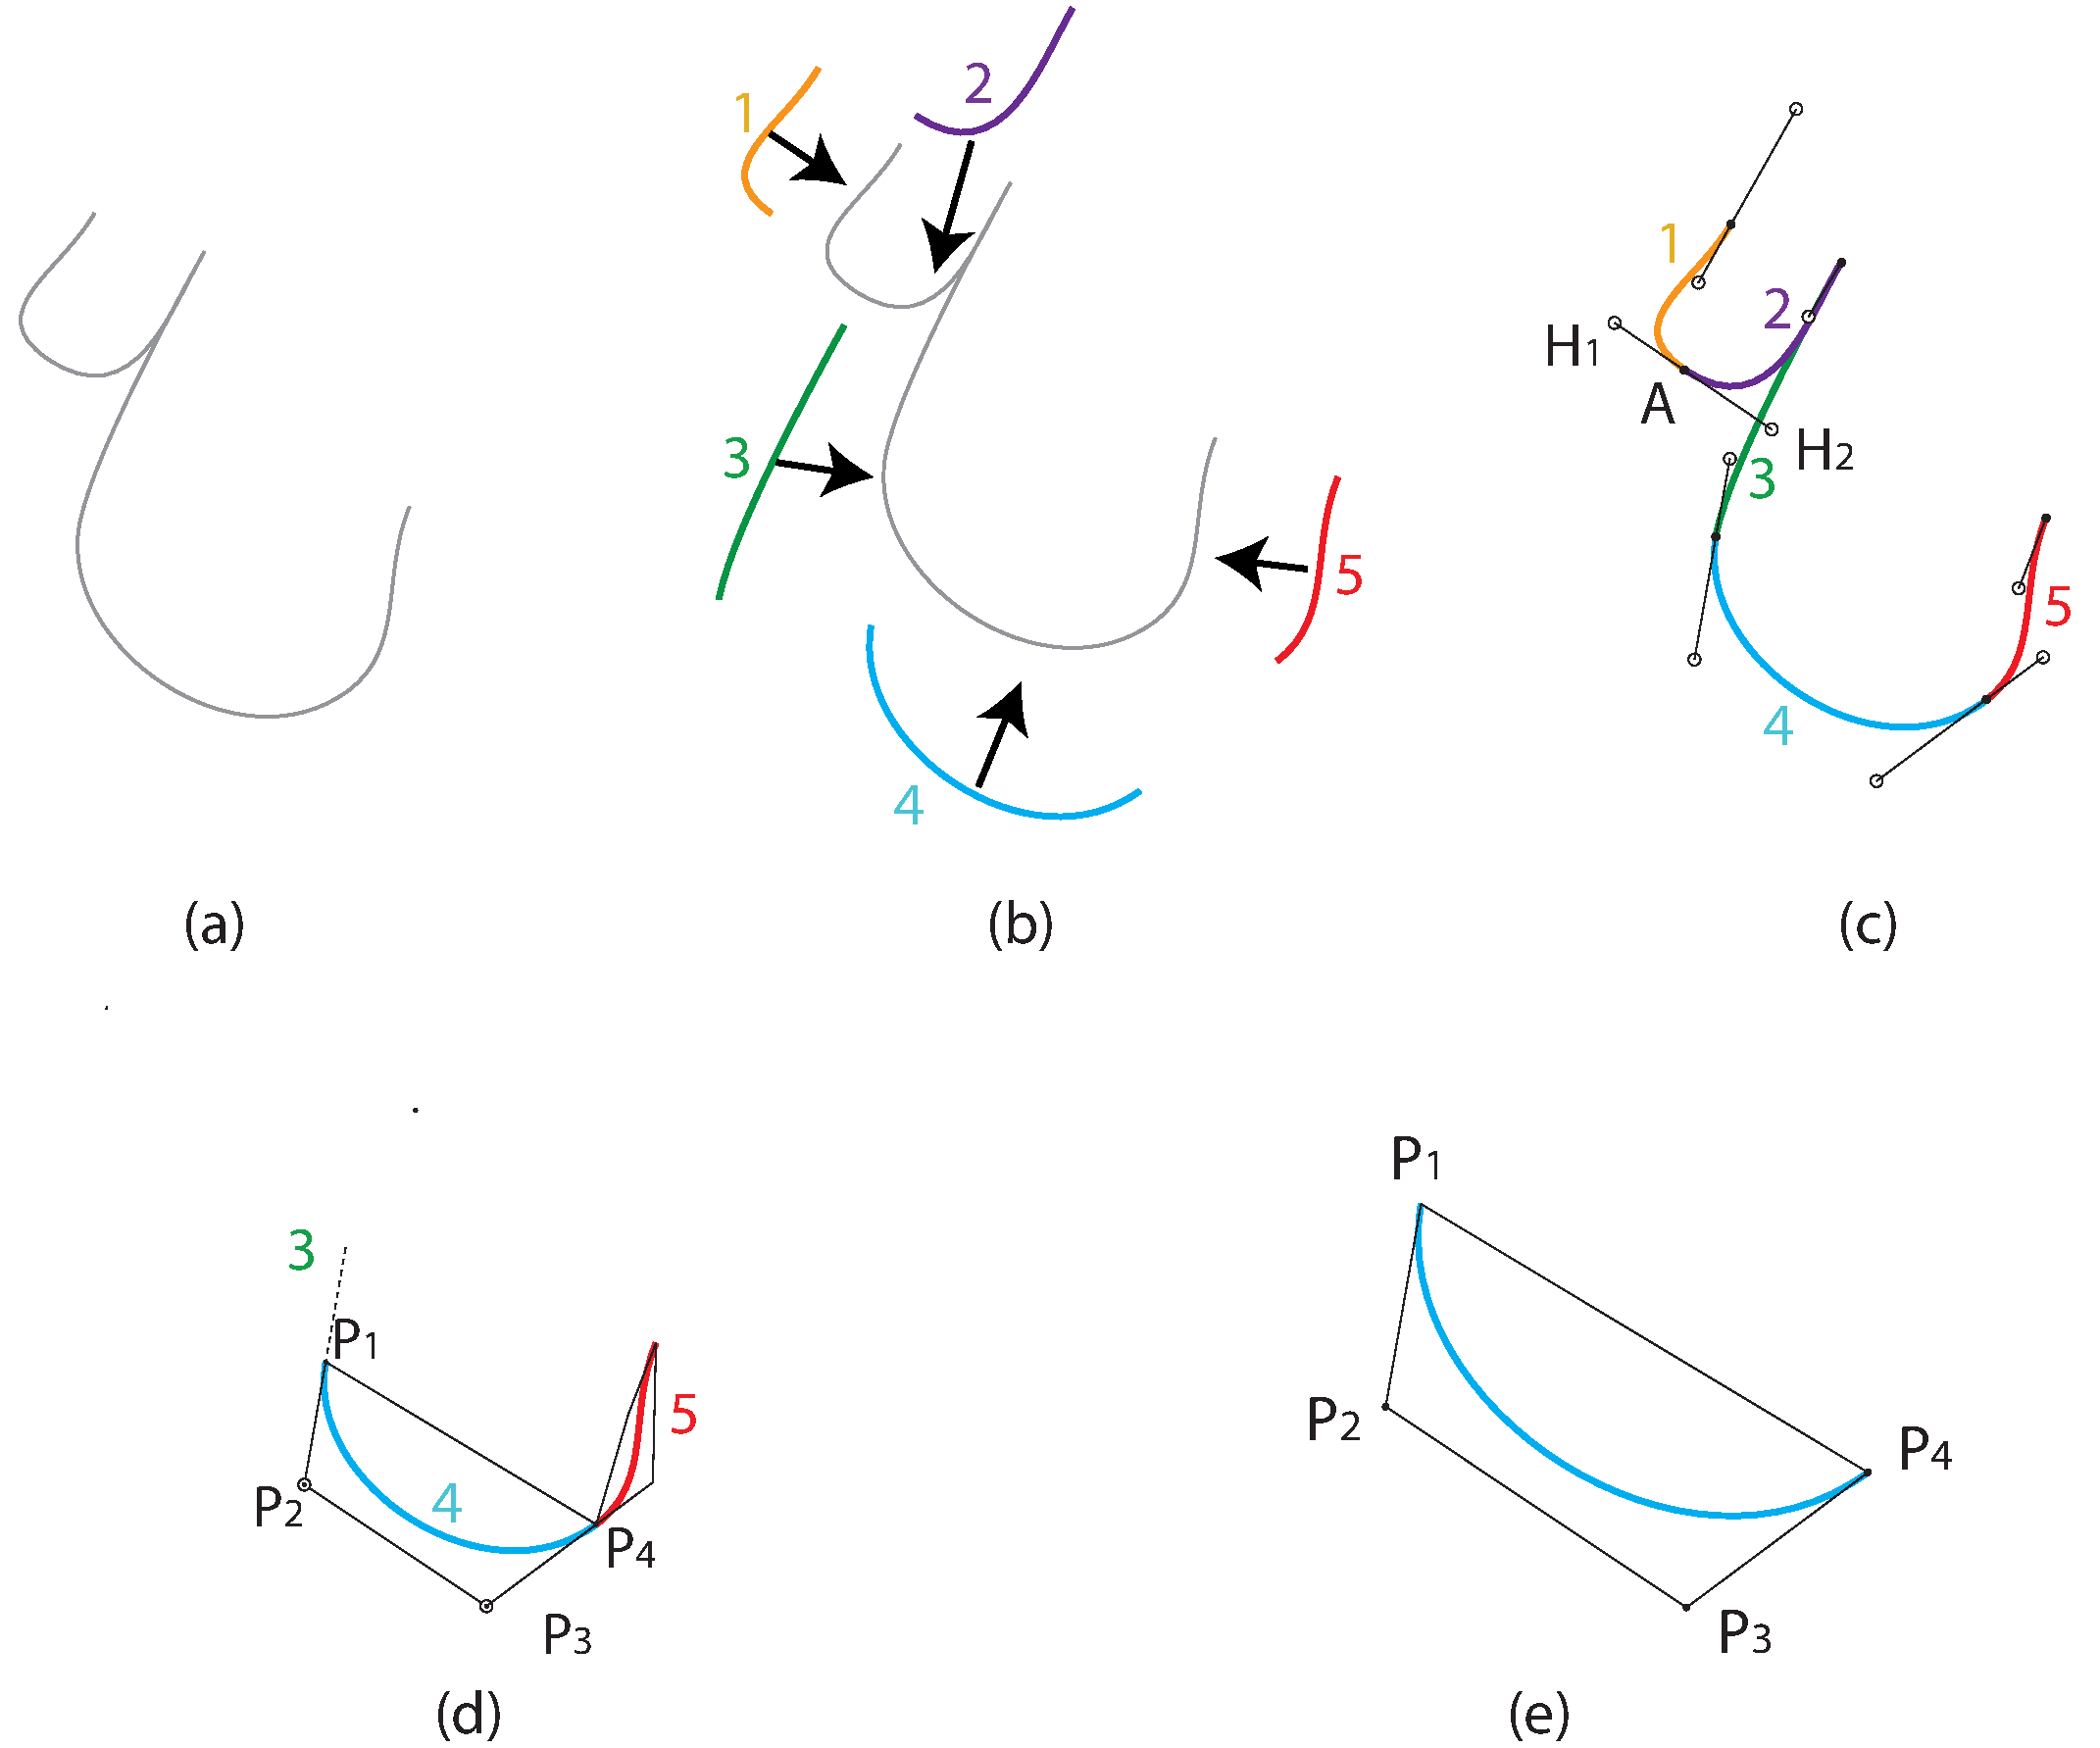
\includegraphics[width=2.5in]{../Images/BezierSplineCurve.pdf}
            \caption{An illustration showing the construction of Bezier Spline Curve. (a) A sample of a Bezier spline path (b) an exploded view of inner curves of the Bezier spline path (c) Handles that control the shape of the two adjacent sub curves (d) and (e) Construction polygon of the sub curve.}
            \label{Fig:BezierSplines}
        \end{figure}

        Now, it may look like the shapes defined in this way are pretty organic but in fact, the whole shape is defined by simple mathematical equations. Figure \ref{Fig:BezierSplines} (d) focuses on section $4$ and $5$ of the curve and also shows a polygon defined by the points $P_1$, $P_2$, $P_3$ and  $P_4$. It must be noted that the points $P_1$ and $P_4$ of this polygon are also the anchor point between sections $3$, $4$ and $5$. Take section $4$ for example here. The polygon mathematically defines the complete shape of this curve part. If $P_{spline}$ is a point on the section $4$, with coordinates $x$ and $y$ in a cartesian plane with some origin, it is defined as
         \begin{equation}
         P_{spline}=P_b×f+P_a×(1 -f).
         \end{equation}
where,
\begin{equation}
P_a=P_{23}×f+P_{12}×(1 -f)
\end{equation}
and
\begin{equation}
P_b=P_{34}×f+P_{23}×(1 -f)
\end{equation}
where,
\begin{align}
P_{12}&=P_2×f+P_1×(1 -f), \\
P_{23}&=P_3×f+P_2×(1 -f)
\end{align}
and
\begin{equation}
P_{34}=P_4×f+P_3×(1 -f)
\end{equation}
for an $f$ in the range $[0, 1]$.

It can also be proved that the side segments of the polygon $\overline{P_1 P_2}$ and $\overline{P_3 P_4}$ are tangent to the curve at the point they meet it at $P_1$ and $P_4$ respectively.


\subsubsection{Twist/Rotation Handle}
    On top of the conventional Bezier splines that work around anchor points that have curvature handles, we add a “Rotation”/”Twist” handle in the anchor and a thickness parameter to the whole curve. A rotation handle is similar to the curvature handle discussed earlier, except it does not have any effect on the shape of the curve. The thickness parameter defines the size of a flat line segment  centered on $P_{spline}$ and sweeping on it. The orientation of this sweeping line is the same as the angle between the twist handle and the respective anchor. See Figure \ref{Fig:RotatingBezierSplines} (a) that shows rotation handles added in the example under discussion. It must be noted that the curvature of the spline remains the same after adding twist handles that are lying horizontally yet. We then add thickness to the curve in Figure \ref{Fig:RotatingBezierSplines} (b). The resulting curve may look a little out of order but it is normal. This is because the rotation handles are lying on their default position. The twist handles may be given some length but it is insignificant since the twist of the curve will only take the value of the angle the handle subtends about the anchor. Figure \ref{Fig:RotatingBezierSplines} (c) shows the final form of the twisting bezier spline after the twist handles have been iteratively moved to position that give the spline the desired look.
        

    In simpler words, it’s similar to sweeping a pen centered on the actual spline while twisting it uniformly and continuously about its own axis according to the equation
    \begin{equation}
    \theta_{twist}=\theta_A  (1-f)+ \theta_B
    \end{equation}
    where $f$ is the same factor that was used to define $P_{spline}$ and $\theta_A$ and $\theta_B$ are the angles between the first and the second anchor and their rotation handles respectively. It may be noted that since each anchor is connecting two adjacent sub curves, the ending angle of the sweeping line at the end of the first curve is always the same at the beginning of the later. This visually hides the transition of the twisting curve from one sub curve to the other.

    It must also be noted that the angle of rotation handle cannot be constrained in a $2\pi$ domain. Instead, it is completely unbounded, and the sweeping pen may actually take multiple turns both clockwise and anticlockwise while moving on a single curve section as well as the whole curve. When the idea of the twisting splines was first conceived, it wasn’t envisaged that the angle had to be taken like in this scheme. Special care had to be taken in order to graphically read a continuous angle from the user.

    See Appendix \ref{Appendix:CodeSnippets} which compiles the rectangular coordinates of all the anchors of the rotating bezier spline shown formatted in a manner that Gregor can interpret. In chapter \ref{Chapter:Gregor}, we discuss in detail ``Gregor'', the tool that uses this data to save the created splines.

    \subsection{Conversion of Existing Calligraphy Artwork}
    Instead of using image processing to extract data from existing scans and photographs of the artworks, using rotating Bezier splines we can now include the artists in the process. Just like any other computer-based graphics design application, we share a proof of concept tool to create, modify, save, and reload rotating Bezier splines. The tool can be downloaded online [link to source][link to user manual] and features an easy to use interface and the tools needed to conveniently create, modify new splines and trace existing ones.

    \subsection{Machine Data Generation}
    \label{ExplorationPoints1}
    The rotating spline curves are themselves emulated ink-marks of a broad edge marking tool. This is the reason extracting machine data and even G-codes from them becomes natural. If the flat side of the tool is assumed to be entirely touching the writing surface, the minimum information required to draw a stroke trickles down to the line on which the pen must move and the twist of the pen in world coordinates. Minus the information about a three dimensional reference system, this is exactly the information a rotating Bezier spline contains once an artist has drawn them on the computer screen. In other words, to call the rotation Bezier splines the machine data, the following assumptions must be made:

    \begin{itemize}
        \item The flat tip of a broad edge tool is always completely touching the drawing area.
    	\item The inclination of the pen with respect to the drawing area or with respect to the direction of the drawing is either normal or always fixed at an angle and is set by the machine.
    	\item To produce thinner strokes, another spline will be used. This means that the machine would have to use multiple tools for such splines.
    	\item The axial pressure the pen inserts on the drawing board while drawing is also fixed and is set by the machine as well.
    
    \end{itemize}

    It is now obvious that to remove the limitations of fixed angles and pressure values, one can add more handles similar to the rotation handle. A set of bi-directional inclination handles can be added right away with a three-dimensional pen position visualizer to assist the artist determine what angle they want to keep the pen at while drawing a specific stroke. The pressure angle, however, would not be recommended without interfacing some hardware that lets the artist feel the pen pressure in real time before setting a handle value. This can be done using a pressure sensitive digital pen or writing tablets [16-18]. These expansions alone are in themselves worthy of research projects that rivals the scope of the current one.

    \section{Performance and Bechmarking}
\label{Chapter:Performance}

\subsection{Characterization}
An important aspect of fabricating a new technique is measuring how well it performs in different usage scenarios. The problem is, in terms of arts, not every mistake the technique makes can be regarded as an issue. Developing a metrics for judging the artistic quality of a calligraphy specimen produced by the Bezier or rotating Bezier splines is altogether a separate discussion and out of scope of this research. However, there are some aspects that we have tried to measure that give us some idea how effective the rotating Bezier splines can be.

\subsection{Supported Scripts}
By ``supported scripts'' one may imply deriving a mathematical model for a particular font or a scipt family. The mainline scripts used in calligraphy are not necessarily as mathematical as the model of the rotating Bezier splines. Especially, when the artists start to utilize their writing tool in unique ways to extract some unique value from the scripts they create, forming a mathematical model becomes practically impossible. However, since in the first place, it would be an artist who will be creating and tracing scripts on the screen of a computer, it is safe to claim that given the similarity of the emulation, rotating Bezier splines can be used to produce any script that is written with broad edge tools. However, these are some limitations inherited by this statement:

\begin{itemize}
\item If the tool changes thickness during a stroke (like a flexible brush), the best alternate to achieve a similar appearance of the script would be to use multiple splines with multiple thicknesses that overlap each other in a gradual manner.
\item Although the rotating splines have a defined tool width, we still assume the tool to be infinitely thin on the other side, more like a narrow line. This makes negligible but still some difference when the virtual tool is replaced with an actual tool. One way to overcome this issue would to come up with another rendering algorithm that also asks for this missing information. This has been discussed in later chapters when we suggest some other improvements in the overall project.
\end{itemize}

\subsubsection{Coverage}
To benchmark the performance and accuracy  of rotating bezier splines, some test results are presented here. These values are produced by comparing high resolution binary images of actual scripts, extracted with Adobe Photoshop and rasterized images produced by the twisting bezier splines produced by tracing the processed images. One-to-one pixel comparison was made using computer scripts to measure the fraction of ink that maps exactly on the original script, lies outside it or is completely missing. Table \ref{Table:Accuracy} presents some values that give some idea of efficacy of the proposed bezier splines.

\begin{table}
\begin{center}
\caption{Benchmark of the mathematical accuracy of the twisting bezier spline curves}
\label{Table:Accuracy}
\begin{tabular}{| c | c |}
  \hline
\textbf{Metrics} & \textbf{Results} \\
  \hline
Area over flow & $<$ 2\% \\
  \hline
Coverage & $>$ $94\%$ \\
  \hline
Lateral deviation from the pitch line & N.A. \\
  \hline
Compatibility & All broad edge scripts \\
  \hline
Total splines measured & $>100$ \\
  \hline
Total pixels compared & $9.9$~million \\
  \hline
Tested scripts & Nastaleeq, Thuluth \\
\hline
\end{tabular}
\end{center}
\end{table}
%
%This metrics is comprehensive but still not complete. Some additional metrices are still needed to give a verdict about how good the proposed solution is and it is now up to the community to evolve these curves according to the needs. Table \ref{Table:AdvancedMetrices} presents a couple of those metrices that may also be desired by the researchers.
%
%\begin{table}
%\begin{center}
%\caption{Advanced metrices to gauge the effectiveness of twisting bezier splines.}
%\label{Table:AdvancedMetrices}
%\begin{tabular}{| c | c |}
%  \hline
%  \textbf{Metrics} & \textbf{How can it be measured} \\
%  \hline
%Easy of usage & A survey based on Likert scale \\
%  \hline
%Time efficiency of tracing & Comparison of the time taken by the same artists tracing with conventional and rotating Bezier splines \\
%  \hline
%The artistic quality of the specimens produces. & A survey based on Likert scale and filled by a wide range of artists \\
%  \hline
%\end{tabular}
%\end{center}
%\end{table}

Please note that the third metrics in Table \ref{Table:AdvancedMetrices} seems potent for gauging the performance of atypical supline but is no longer valid given the nature of fabricated splines.

\subsubsection{Sample Results}
As a test and a tribute, two scripts by the famous teacher, artist and author of $18$ calligraphy books, late Khursheed Gohar Qalam \cite{bib23} of the National College of Arts (NCA) were borrowed; one in Nastaleeq and other in Thuluth. Figure \ref{Fig:InkComparison} shows a detailed comparison of a part of a famous script produced by Gohar with the version traced with twisting bezier splines. The comparison unveils how accurately the bezier splines appear to be tracing the original script. The original appearing in Figure \ref{Fig:InkComparison}(a) image is first processed to be used with the spline editor and then converted to a binary image which is shown in Figure \ref{Fig:InkComparison}(b). Figure appearing in Figure \ref{Fig:InkComparison}(c), (d) and (e) are then produced by rasterizing the traced spline and a one-to-one pixel comparison of both images. See Table \ref{Table:AdvancedMetrices} which shows a quantitative measure of the trace accuracy. With these values, it is fair to assert that the twisting splines are very accurately mimicking the original sample.

However no matter how accurate they look, it must also be noted that since the original image is not available in a sufficiently high digital resolution, strictly speaking, Figure \ref{Fig:InkComparison}(d) and (e) do not do not show the true picture of the error that the curves produce but only a reasonably good estimate. The final verdict about the accuracy can only be given in form of the appeal this technique gets when actually presented in the community.

Figure \ref{Fig:Nastaleeq} and \ref{Fig:Thuluth} show sample outputs produced by tracing two of famous Gohar's articles in ``Nastaleeq'' and ``Thuluth'' scripts. The twisting splines do contain vector data and have no resolution but for the sake of presentation, the images have been rasterized by ``Gregor''.

    \begin{figure}[!t]
        \centering
        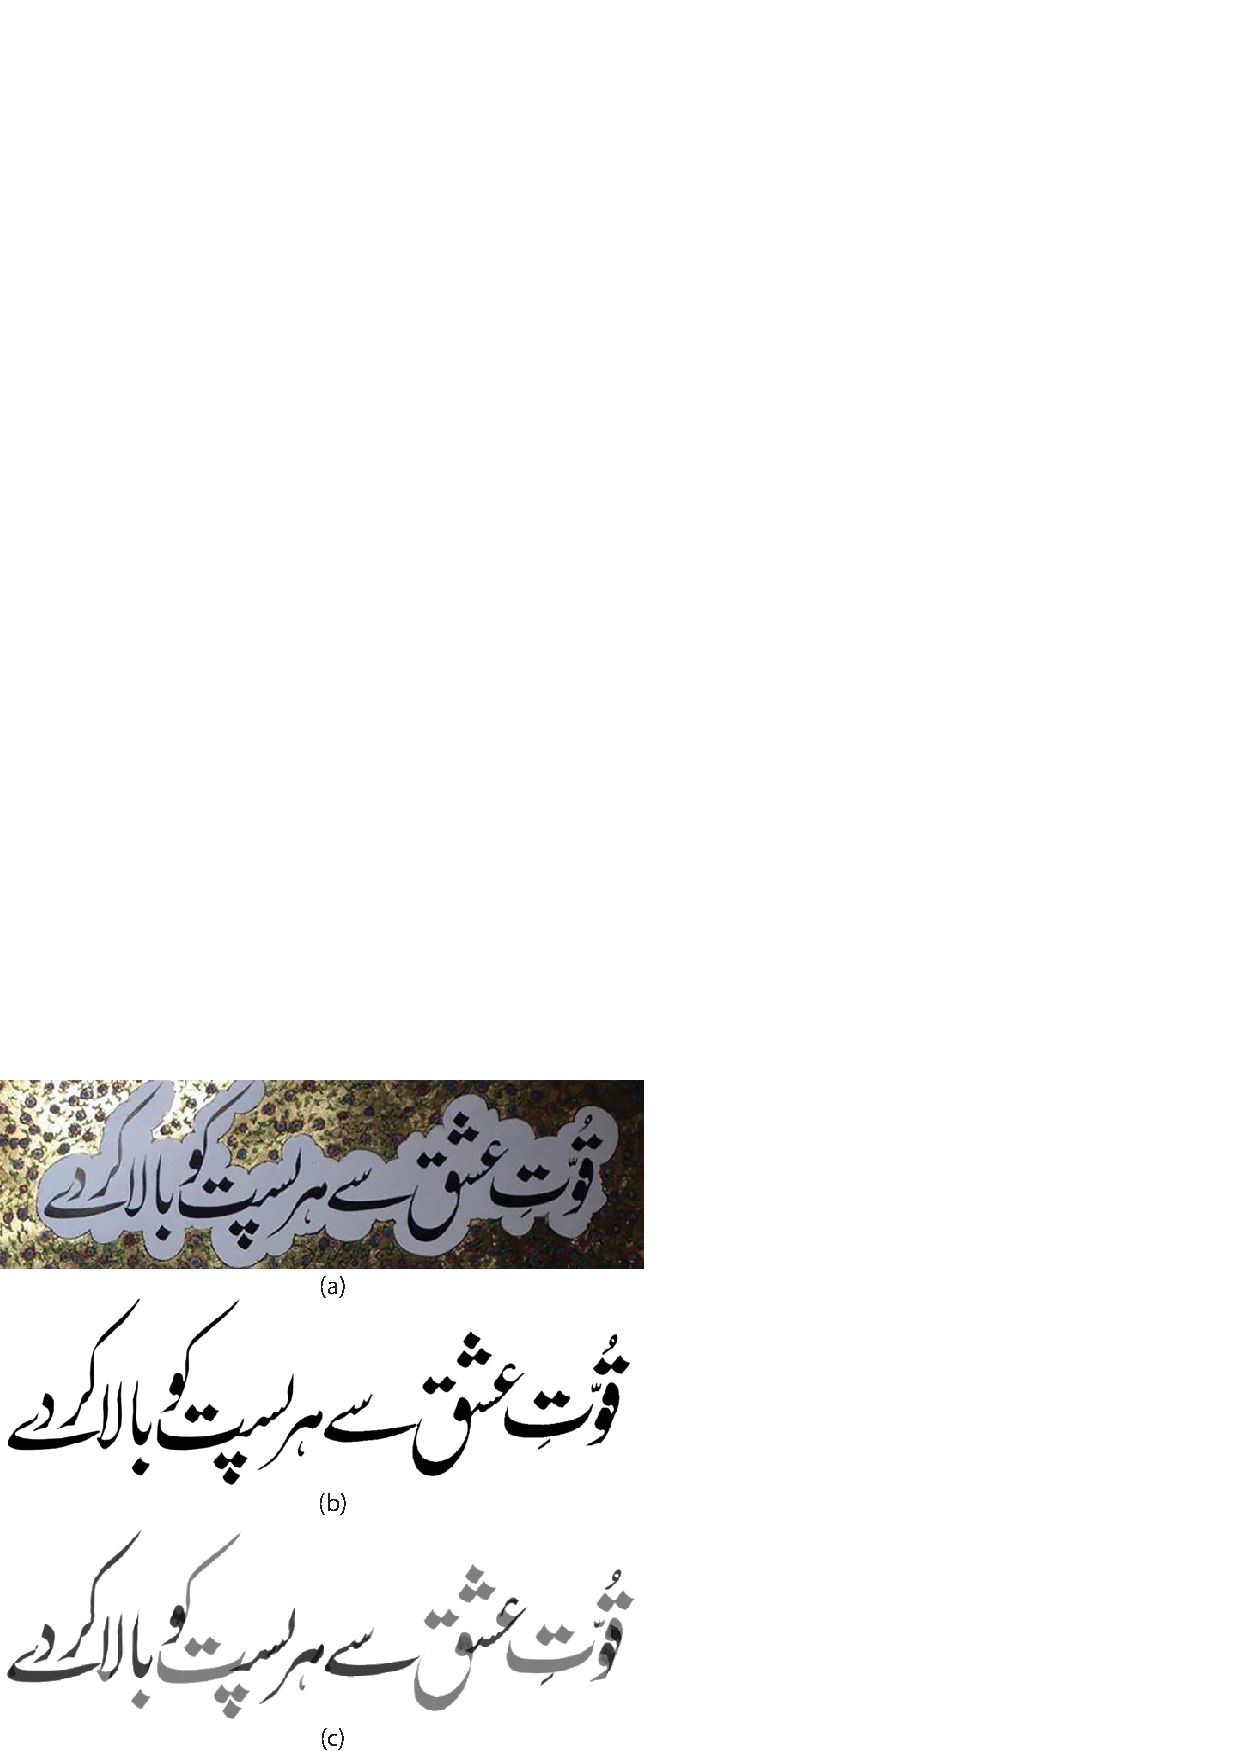
\includegraphics[width=2.5in]{../Images/NastaleeqSample.pdf}
      \caption{
        A specimen produced in ``Nastaleeq'' script. (a) Original photograph of the specimen (b) Rasterized binary image of the twisting spline curves. (c) Rasteriezd shaded image of the twisting spline curves highlighting individual curve parts.}
      \label{Fig:Nastaleeq}
    \end{figure}


    \begin{figure}[!t]
    \centering
    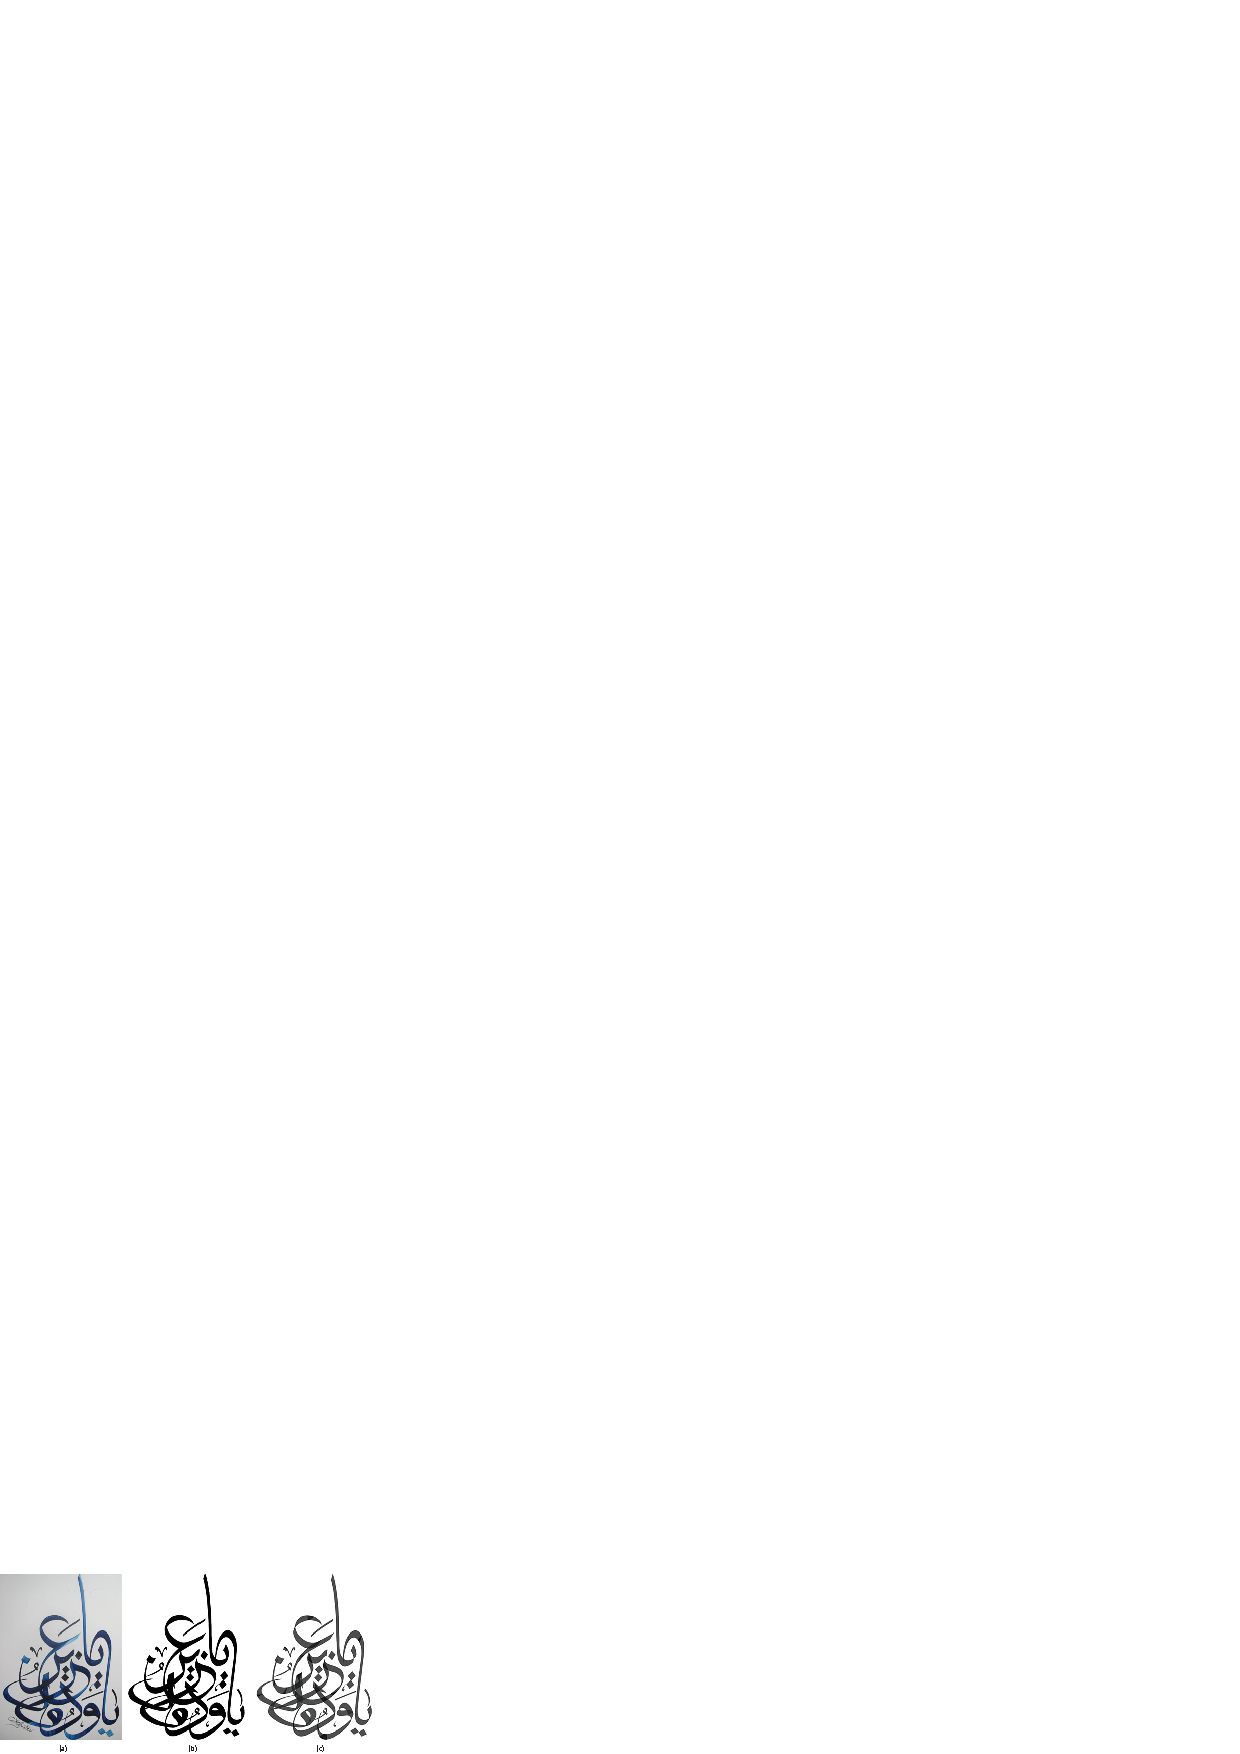
\includegraphics[width=2.5in]{../Images/ThuluthSample.pdf}
    \caption{
        A specimen produced in ``Thuluth'' script. (a) Original photograph of the specimen (b) Rasterized binary image of the twisting spline curves. (c) Rasteriezd shaded image of the twisting spline curves highlighting individual curve parts.
    }
  \label{Fig:Thuluth}
\end{figure}

\subsubsection{Machine Data Generation and Simulation}
    To check how accurately the data generated by these splines can be traced by an actual robotic manipulator, computer simulation was used. We use an open-source simulator, developed in-house for the task. The simulator can simulate a $6$~DoF robotic manipulator with on-screen $3$D visualization.

    Using the same model of the spline model, the simulator first rasterizes the whole spline and then transforms the two dimensional points onto a plannar surface simulated on a user desired position in the workspace. Then it creates a pseudo machine code to mimic the tool changes required before each stroke and the transformed rasterized points are directly considered as G-Codes for the manipulator. Once computed it starts implementing the program.

    For the sake of analysis, in parallel, the end effector orientation is captured continuously to construct an ink mark with each sweep of the tool. The reproduced image is then used for analysis. The results of such a comparison can be seen in Table \ref{Table:MachineDataMetrices}. The value indicate that the robot very closely reproduces the given spline thus verifying the thesis of the research.

    \begin{table}
    \begin{center}
    \caption{Benchmark of the mathematical accuracy of the twisting bezier spline curves with a simulated manipulator}
    \label{Table:MachineDataMetrices}
    \begin{tabular}{| c | c | c | c |}
    \hline
      & \textbf{Reference} & \textbf{Coverage} & \textbf{Extra} \\
      \hline
      \multicolumn{4}{|l|}{\textbf{Nastaleeq}}\\
      \hline
      Rotating Bazier Spline & Original Image & 95.8\% & 5.4\% \\
      \hline
      Machined Output & Original Image & 96.7\% & 7.0\% \\
      \hline
      Machined Output & Rasterized Image & 96.7\% & 4.3\% \\
      \hline
      \multicolumn{4}{|l|}{\textbf{Thuluth}}\\
      \hline
      Rotating Bazier Spline & Original Image & 93.4\% & 2.8\% \\
      \hline
      Machined Output & Original Image & 95.0\% & 3.4\% \\
      \hline
      Machined Output & Rasterized Image & 97.8\% & 4.4\% \\
    \hline
    \end{tabular}
    \end{center}
    \end{table}        % Twisting Bezier Splines
    \section{Conclusion}
\label{Chapter:Conclusion}
{
    The twisting Bezier spline curves very closely mimic the ink mark of broad edge tools thus creating very accurate calligraphy scripts as seen in Figure \ref{Image:spline_prev}. With most of broad edge scripts, on an average, they give more than 95\% coverage of the reference image an less than 5\% overdraw. This has now been verified by comparing them with original calligraphy specimens as well as after simulating the output of a robotic manipulator.

    \begin{figure}[!t]
        \centering
        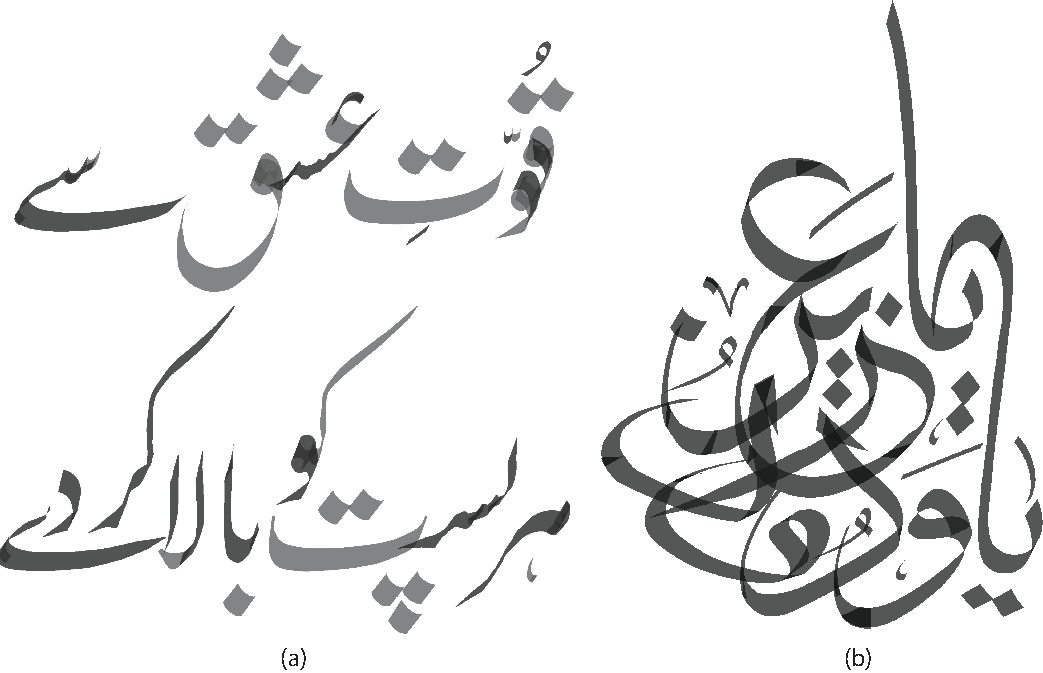
\includegraphics[width=2.5in]{../Images/rotating bezier splines preview.pdf}
      \caption{A preview of the calligraphy produced using the rotating bezier splines.
      } \label{Image:spline_prev}
    \end{figure}

    With tools created as a by-product of this research, an artist can not only trace existing calligraphy scripts, but also create and modify new ones with a very lean learning curve. The ease of use of the tools created for the tast assures that the focus of the artist is more on the art itself than the caveats of the software solution.

    Where the accuracy of the splines has been characterised and ease of use has been demonstrated, there still are a lot of unexplored areas that require more research. As discussed in section \ref{ExplorationPoints1}, one can pack the tool inclination and normal pressure information into the rotating splines. One can also choose to implement other kinds of manipulators and actuators to test the performance of the splines in the simulator. Last but not the least, since the simulator can emulate a pseudo robot, it can also be modified to be used as a live controller for a real robotic manipulator.

    While this thesis puts together the results of some crucial tests to establish the usefulness of rotating splines, the final verdict will still be given by the community that takes the work forward in more scenarios and conditions.
}
    \begin{thebibliography}{99}
\bibitem{bib01} Web page of Baytulhabeeb, an artist, \url{https://bit.ly/islamic_cal_history}, accessed on Sep 4, 2020.
\bibitem{bib02} Arabetics™, a private foundry and consulting firm, specializing in Arabic type and lettering designs, “Roots of Modern Arabic Script:  From Musnad to Jazm”, \url{https://bit.ly/islamic_cal_history_2}, accessed on Sep 4, 2020.
\bibitem{bib03} “Islamic Calligraphy”, \url{https://bit.ly/Islamic_cal_wiki}, accessed on Sep 4, 2020.
\bibitem{bib04} By Julia Kaestle , “Arabic calligraphy as a typographic exercise”, \url{https://bit.ly/cal_styles}, accessed on Sep 4, 2020.
\bibitem{bib05} Haji Noor Den, Portfolio, \url{http://www.hajinoordeen.com/about.html}, accessed on Sep 4, 2020.
\bibitem{bib06} Mohammad Zakrya, Portfolio, \url{https://mohamedzakariya.com}, accessed on Sep 4, 2020.
\bibitem{bib07} Kamel Al Baba, Mokhtar Al Baba, Portfolio, \url{http://www.arabiccalligraphy.com}, accessed on Sep 4, 2020.
\bibitem{bib08} Abed Yaman, “A look at the history of Arabic calligraphy” \url{https://bit.ly/islamic_cal_stages}, accessed on Sep 4, 2020.
\bibitem{bib09} M. A.-de Lemos, and E. V. Liberado, “Industrial robotics applied to education”, Proceedings of 2011 International Conference on Computer Science and Network Technology.
\bibitem{bib10} Robotics in Agriculture: Types and Applications, \url{https://bit.ly/ind_robots_in_agri}, accessed on Sep 4, 2020.
\bibitem{bib11} A robot playing table tennis, \url{https://www.kuka.com/timo}, accessed on Sep 4, 2020.
\bibitem{bib12} A printing robot, \url{https://bit.ly/ind_robot_cal}, accessed on Sep 4, 2020.
\bibitem{bib20} Project code repository on GitHub, \url{https://github.com/umartechboy/Thesis_2017-MS-MC-17}|, accessed on August 8, 2021.
\bibitem{bib13} M. Bilal, A. Raza, M. Rizwan, M. Ahsan, H. F. Maqbool, S. Abbas Zilqurnain Naqvi, “Towards Rehabilitation of Mughal Era Historical Places using 7 DOF Robotic Manipulator”, in Proceedings, IEEE International Conference on Robotics and Automation in Industry, pp. 1-6, 2019.
\bibitem{bib14} GIMP, GNU Image Manipulation Program Developers Resources, \url{https://bit.ly/gimp_developers}, accessed on July 7, 2021.
\bibitem{bib15} Inkscape Extensions, \url{https://bit.ly/inkscape_developers}, accessed on July 7, 2021.
\bibitem{bib16} Wacom Intuos, \url{https://bit.ly/wacom_intuos_official}, accessed on July 7, 2021.
\bibitem{bib17} Lenovo Thinkpad x380, \url{https://bit.ly/lenovo_thinkpad_x380}, accessed on July 7, 2021.
\bibitem{bib18} Microsoft Surface Pro 7, \url{https://bit.ly/ms_surface_pro_7}|, accessed on July 7, 2021.
\bibitem{bib19} George R. R. Martin, \emph{``A Game of Thrones''}, Chapter $30$.
\bibitem{bib21} \emph{Solving a 6 DoF Robot}, \url{https://bit.ly/SolvingA6DoFRobot}, accessed on November 30, 2021.
\bibitem{bib22} Microsoft .Net Framework, \url{https://bit.ly/ms_dotnet_framework}, accessed on Jan 09, 2022.
\bibitem{bib23} Khursheed Gohar Qalam, \url{https://bit.ly/gohar_qalam}, accessed on Jan 09, 2022.
    \end{thebibliography} 
% uncomment to enable review format
%\end{paracol}
\end{document}


